%!TEX root = ../hutbthesis_main.tex

\clearpage
\thispagestyle{empty}
\begin{center}
{\fontsize{22pt}{28pt}\selectfont\heiti 湖南工商大学本科毕业设计}\par
\vspace{1.2cm}
{\fontsize{22pt}{28pt}\selectfont\heiti 版权使用授权书}\par
\end{center}

\vspace{1.0cm}
\setlength{\parindent}{2em}
{\fontsize{14pt}{24pt}\selectfont\songti
本毕业论文《基于模拟器的极端驾驶仿真场景的生成算法研究》是本人在校期间所完成学业的组成部分，是在学校教师的指导下完成的。因此，本人特授权学校可将本毕业设计的全部或部分内容编入有关书籍、数据库保存，可采用复制、印刷、网页制作等方式将设计文本和经过编辑、批注等处理的设计文本提供给读者查阅、参考，可向有关学术部门和国家有关教育主管部门呈送复印件和电子文档。本毕业设计无论做何种处理，必须尊重本人的著作权，署明本人姓名。
\par}

\vfill
\begin{flushright}
{\fontsize{14pt}{22pt}\selectfont\songti
\begin{tabular}{rlcl}
设计作者（签字）： & 
\includegraphics[height=1.3cm,keepaspectratio]{images/auth_author.png} & \hspace{1.5cm} 时间 & 2026年5月25日 \\[1.2cm]
指导教师已阅（签字）： &
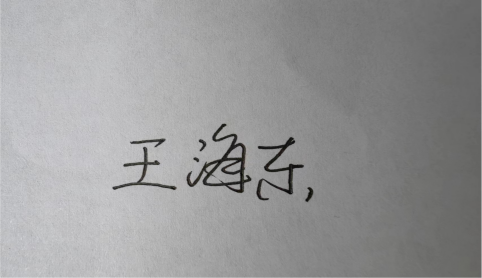
\includegraphics[height=1.4cm,keepaspectratio]{images/auth_teacher.png} &
\hspace{1.5cm}时间 & 2026年5月25日 \\
\end{tabular}}
\end{flushright}
\clearpage
